\documentclass[conference]{IEEEtran}
\IEEEoverridecommandlockouts
% The preceding line is only needed to identify funding in the first footnote. If that is unneeded, please comment it out.
\usepackage{cite}
\usepackage{amsmath,amssymb,amsfonts}
% \usepackage{algorithm}      % clashes with algorithm2e -- not needed any more
% \usepackage{algorithmic}
% \usepackage{algpseudocode}  % clashes with algorithm2e -- not needed any more
\usepackage{graphicx}
\usepackage{textcomp}
\usepackage{xcolor}
\usepackage[hidelinks]{hyperref}
\usepackage{float}
\usepackage{booktabs}
\usepackage{pgfplots}
\usepackage{placeins}
\usepackage{balance}
\usepackage[ruled,vlined,linesnumbered]{algorithm2e}
\usepackage{tikz}
\usetikzlibrary{positioning,calc,arrows.meta,shapes.geometric,fit,backgrounds}
\pgfplotsset{compat=1.18}
\newcommand{\missing}[1]{\textit{#1}}
\def\BibTeX{{\rm B\kern-.05em{\sc i\kern-.025em b}\kern-.08em
    T\kern-.1667em\lower.7ex\hbox{E}\kern-.125emX}}
\begin{document}


\title{
\fontsize{22}{25}\selectfont
CodeSheriff: Design and Development of an Agentic Security
Auditor for an SFI-Enabled Confidential CI/CD Execution
Layer Using Bayesian Vulnerability Inference
}

\author{\IEEEauthorblockN{Shubhankar Vishnu Patil}
\IEEEauthorblockA{\textit{Dept. of Information Technology} \\
\textit{G H Raisoni College of Engineering and Management}\\
Pune, India \\
shubhankarp258@gmail.com}
\and
\IEEEauthorblockN{Vivek Dnyaneshwar Joshi}
\IEEEauthorblockA{\textit{Dept. of Information Technology} \\
\textit{G H Raisoni College of Engineering and Management}\\
Pune, India \\
vivekdjoshi05@gmail.com}
\and
\IEEEauthorblockN{Yash Suresh Kodgirwar}
\IEEEauthorblockA{\textit{Dept. of Information Technology} \\
\textit{G H Raisoni College of Engineering and Management}\\
Pune, India \\
yashkodgirwar@gmail.com}
\and
\IEEEauthorblockN{Nirmalya Mukhopadhyay}
\IEEEauthorblockA{\textit{Dept. of Information Technology} \\
\textit{G H Raisoni College of Engineering and Management}\\
Pune, India \\
}
\and
\IEEEauthorblockN{Kunal Kundu}
\IEEEauthorblockA{\textit{Dept. of Information Technology} \\
\textit{G H Raisoni College of Engineering and Management}\\
Pune, India \\
}
}

\maketitle

\begin{abstract}
Modern software development increasingly relies on Continuous
Integration/Continuous Deployment (CI/CD) pipelines to deliver software
rapidly, but automated security review at the pull request stage remains
limited. Existing security tools rely on rigid static analysis or
homogeneous multi-agent approaches, which may generate false positives or
overlook complex vulnerabilities, and they report a verdict without any
measure of how often that verdict is right. This paper presents
CodeSheriff, an agentic security auditor that analyzes GitHub pull requests
using structural, semantic, contextual, and SFI-based confidential
execution analysis. A Bayesian inference engine fuses evidence from the
four agents into a calibrated vulnerability probability, and an automated
patch generation and verification module recommends and validates fixes
through GitHub and a web dashboard. On a labelled corpus of 76 Python
functions arranged as 38 vulnerable--safe twin pairs, CodeSheriff attains
an $F_1$ of $0.923$ at a precision of $1.000$ with an expected calibration
error of $0.027$, while majority voting over identical agent evidence
attains an $F_1$ of only $0.142$ at five times the calibration error. The
system therefore delivers reliable, explainable, and statistically grounded
vulnerability detection while reducing manual review effort.
\end{abstract}
\vspace{6pt}
\begin{IEEEkeywords}
vulnerability detection, multi-agent systems, software security, Bayesian
inference, probability calibration, software fault isolation, continuous
integration and continuous deployment
\end{IEEEkeywords}


\section{Introduction}
In today’s software industry, developers frequently push code to the main branch through Pull Requests (PRs). However, security analysis of each Pull Request is still largely performed manually, making the review process more time-consuming.Teams either use basic approaches that only catch known, simple mistakes, or they don't have enough time to properly review every pull request. This is a big problem because even one missed vulnerability can put the whole application at risk once the code is merged and deployed. On top of this, attackers are now also targeting the Continuous Integration/Continuous Deployment (CI/CD) that's builds and runs the code.

Solutions that exist today don’t fully solve this problem. Traditional static analysis approaches identify fixed patterns but are unable to catch tricky ones, so they generate a lot of false alarms. Some recent tools use multiple artificial intelligence (AI) agents, but all these agents basically read the same code in the same way, so they don't really give different opinions. when these approaches combine results, they just use simple voting, which doesn't tell you how confident the final answer actually is.

In this paper, we are proposing CodeSheriff to fix this problem. It uses four different types of agents that look at the code from different perspectives. Static agent checks the code structure, the meaning of the code is understood by the semantic agent, the context agent checks whether accepting this PR could bring back any vulnerability from previously accepted PR, and the runtime agent actually watches the code run inside a safe, isolated environment using software fault isolation (SFI). All this information is then combined using a Bayesian model, which gives a clear probability of whether the code is vulnerable, along with how confident the system is. This same safe environment also protects the CI/CD workflow, since it only releases secret keys when it is sure the correct, verified code is running.


The rest of this paper is structured as follows. Section \ref{LS} talks
about related work already done in this area. Section \ref{PS} explains our
proposed method, its mathematical model, algorithms and workflow.
Section \ref{IMP} describes the implementation. Section \ref{RES} reports
and discusses the results, and Section \ref{CON} concludes the paper with
the future scope.

\section{Literature Survey} \label{LS}

Early learning-based studies explored structural and sequential representations for vulnerability detection. Li and Yang \cite{ref20} compared sequence and graph-based deep learning methods, identifying challenges in capturing long-range dependencies and generalizing to noisy data. CODE-SMASH \cite{ref19} and XTransformer \cite{ref18} employed hierarchical neural and transformer architectures to capture multi-level code representations and improve similarity-based detection, while remaining sensitive to computational cost and dataset characteristics . Abbasi and Shameli-Sendi \cite{ref4} used Code Property Graph metrics with machine learning for interpretable vulnerability and vulnerability-type prediction, but their approach was limited to C/C++. DeepSecure \cite{ref2} combined CodeBERT with bidirectional long short-term memory(BiLSTM) and convolutional neural network(CNN) layers for python vulnerability detection, incorporating robustness and confidence calibration, but remained language-specific and affected by noisy labels.

Transformer and large language model(LLM) based approaches have subsequently improved semantic analysis of source code. Shestov \textit{et al.} \cite{ref13} fine-tuned WizardCoder using parameter-efficient learning for vulnerability classification, but remained limited to function-level analysis. Tamberg and Bahsi and Gnieciak and Szandala \cite{ref14,ref17} benchmarked LLMs against vulnerability detection tasks and traditional static analysis tools, showing strong potential but persistent false positives, hallucinations, localization errors, and inference costs. Gülmez \cite{ref7} surveyed code-generation LLMs and highlighted challenges in structural correctness, repository-level reasoning, and security. Chen \textit{et al.} \cite{ref9} and Su \textit{et al.} \cite{ref8} similarly identified limitations involving context windows, hallucination, dataset quality, generalization, and interpretability. Germano \textit{et al.} \cite{ref10} reviewed LLM-based vulnerability detection, repair, and explanation, noting that research remains more focused on detection than automated repair and explanation.

To address the limitations of isolated code analysis, recent studies have incorporated contextual and repository-level information. Antal \textit{et al.} \cite{ref3} evaluated retrieval augmented generation (RAG) for real-world Java vulnerability detection using retrieved vulnerable and secure examples, but observed false positives and retrieval sparsity. AegisGuard \cite{ref1} incorporated contextual information for semantic vulnerability detection and risk stratification, while SCOUT\cite{ref5} enabled interactive repository exploration to retrieve relevant code context. Göçmen \textit{et al.} \cite{ref15} integrated repository history and dependency analysis into pull-request reviews for change-impact estimation, although static dependency analysis cannot fully capture dynamic behavior.

Multi-agent approaches have further introduced collaborative security reasoning. Wei \textit{et al.} \cite{ref11} used specialized roles and collaborative reasoning for vulnerability auditing, while MAVUL \cite{ref16} combined vulnerability analysis, security architecture review, and iterative evaluation. Reddy \textit{et al.} \cite{ref6} explored knowledge-based agentic AI for automated vulnerability triage, and Syed \textit{et al.} \cite{ref12} investigated an observe--reason--act--verify framework for autonomous software-supply-chain defense. These studies demonstrate the potential of agentic security workflows, while also highlighting challenges such as reduced performance on complex cases, token overhead, and the need for human intervention.

However, existing approaches do not effectively combine structural, semantic and contextual analysis within a unified vulnerability detection framework. We integrate these approaches through specialized agents and confidence-aware vulnerability inference, while providing explanations and patch recommendations within the GitHub pull-request workflow.

\section{Proposed Methodology} \label{PS}

A vulnerability can hide in the structure of the code, in its intent, in a
departure from the repository's own habits, or only in what the code does
when it runs. CodeSheriff therefore analyses every changed function with
four independent agents -- Structural, Semantic, Context and Runtime --
that never see each other's output, and fuses their evidence by Bayesian
inference instead of voting, so the reported confidence is calibrated
rather than asserted.

\subsection{Mathematical Model}

The framework evaluates a pull request in five stages: change extraction,
independent agent analysis, evidence categorisation, Bayesian fusion and
the alert decision. The unit of analysis is one changed function $u$,
obtained by mapping every line that differs between the base and head
versions of a file to the outermost function containing it.

\subsubsection{Structural Agent}
The Structural Agent follows data through a definition--use graph from each
function parameter, which is treated as untrusted, to a security-sensitive
operation (a \emph{sink}) such as \texttt{cursor.execute} or
\texttt{os.system}, and checks whether the path is sanitized. When an
unsanitized path reaches a sink, the structural score is
\begin{equation}
S_{\mathrm{str}}=\operatorname{clamp}_{[0,1]}\bigl(0.45+\delta+0.15\,\nu-0.25\,\varsigma-0.20\,\tau-\lambda\bigr)
\label{eq:str}
\end{equation}
where $\delta$ is $0.20$ for a critical sink and $0.10$ for a high-severity
sink, $\nu=1$ for a network-facing unit, $\varsigma=1$ when a partial
sanitizer lies on the path, $\tau=1$ in a test file, and $\lambda\le0.05$
is a small penalty for long paths. Semgrep runs as a second backend on the
same unit, and the larger of the two scores is kept, because both read the
same source text with the same technique.

\subsubsection{Semantic Agent}
The Semantic Agent uses a large language model to infer the functional
intent of the code, its trust boundaries and the security invariant that
the change breaks. The model is sampled $n=3$ times with different seeds,
and a sample is accepted only if the weakness class is in scope, the file
matches, the quoted sink appears verbatim in the source and the reported
lines lie inside the unit. For weakness class $c$, the semantic score is
the agreement across accepted samples:
\begin{equation}
S_{\mathrm{sem}}(c)=\frac{m_c}{n}
\label{eq:sem}
\end{equation}
where $m_c$ is the number of accepted samples reporting $c$ and $n$ is the
total number of samples. A single sample cannot separate confidence from
chance, which is why agreement, not the model's own wording, is the score.

\subsubsection{Context Agent}
The Context Agent retrieves the repository's own merged history using local
sentence embeddings stored in pgvector and reports a security control
$\gamma$ that the history applies and the changed function does not. The
contextual score is
\begin{equation}
S_{\mathrm{ctx}}(\gamma)=b\cdot\min\!\Bigl(1,\ \frac{\bar{s}}{0.85}\Bigr)
\label{eq:ctx}
\end{equation}
where $\bar{s}$ is the mean similarity of the retrieved supporting
functions, and $b=0.85$ when the same function established $\gamma$ in an
earlier merge or three or more sibling functions apply it, and $b=0.65$
when exactly two siblings apply it. A single neighbour is treated as
coincidence and reports nothing.

\subsubsection{Runtime Agent}
The Runtime Agent executes the changed function once inside a WebAssembly
sandbox built on Wasmtime and WASI, which enforces software fault isolation
at the instruction level: the network is denied at link time, the
environment is empty and fuel, time and memory are capped. Each parameter
is bound to a unique random token, so a value is untrusted exactly when one
of those tokens appears inside it. If such a value reaches a sink, the
agent reports a detection with the fixed score $S_{\mathrm{rt}}=0.85$, a
constant because this is a direct observation and not an estimate. If the
sink was reached only because the sandbox had to answer a guard it could
not evaluate, the agent abstains.

\subsubsection{Bayesian Fusion and Decision}
Every agent returns a \emph{detection} with a score, a \emph{silence} (it
ran and found nothing) or an \emph{abstention} (it could not run). Raw
scores from different agents are not directly comparable, so each statement
is first mapped to one shared evidence cell:
\begin{equation}
z_a=
\begin{cases}
\textsc{high}, & S_a \ge 0.8\\
\textsc{medium}, & 0.5 \le S_a < 0.8\\
\textsc{low}, & S_a < 0.5\\
\textsc{silence}, & \text{agent ran, found nothing}
\end{cases}
\label{eq:cell}
\end{equation}
Each cell is weighted by how reliably it has predicted vulnerability in
labelled data, through a likelihood ratio estimated with Laplace smoothing:
\begin{equation}
\Lambda_a(z)=\frac{P(z\mid V)}{P(z\mid\neg V)}\approx
\frac{(k_V+1)/(N_V+4)}{(k_S+1)/(N_S+4)}
\label{eq:lr}
\end{equation}
where $k_V$ and $k_S$ are the numbers of vulnerable and safe examples that
fell into cell $z$, and $N_V$ and $N_S$ are the corresponding totals. An
abstention, and any cell never observed, takes $\Lambda_a=1$, so an agent
that could not look leaves the result unchanged instead of being read as a
vote of ``safe''. Ratios are clamped to $[0.05,20]$ so that no single agent
can dominate. The prior odds are then updated multiplicatively and
converted back into a probability:
\begin{equation}
P(V\mid E)=\frac{O}{1+O},\qquad
O=\frac{\pi}{1-\pi}\prod_{a\in\{S,M,C,R\}}\Lambda_a(z_a)
\label{eq:post}
\end{equation}
where $\pi$ is the prior probability of a vulnerability and $O$ is the
posterior odds. The product always contains four factors, one per agent,
and a silence contributes a factor below $1$, so the probability can fall
as well as rise. The finding is finally labelled
\begin{equation}
\mathrm{Verdict}=
\begin{cases}
\textsc{alert}, & P(V\mid E)\ge\tau\\
\textsc{no alert}, & \text{otherwise}
\end{cases}
\label{eq:verdict}
\end{equation}
where $\tau$ is the alert threshold fitted on labelled data. With
$\pi=0.03$ and $\tau=0.227$, one strong semantic detection that no other
agent contradicts is exactly sufficient to alert, while a medium
structural, a high semantic and a high runtime detection together give
$P(V\mid E)\approx0.97$.

\subsection{Algorithms}

The framework is implemented as two algorithmic stages: independent
evidence generation by the four agents, and Bayesian fusion with the alert
decision and patch handoff.

\begin{algorithm}[htbp]
\small
\caption{Agent Evidence Generation}
\label{alg:agents}
\KwIn{Changed function $u$}
\KwOut{Evidence $E=\{e_S,e_M,e_C,e_R\}$}
\ForEach{agent $a \in \{S, M, C, R\}$}{
  \uIf{$a$ cannot analyse $u$}{
    $e_a \gets$ \textsc{Abstention}(reason)\;
  }
  \Else{
    $F_a \gets$ findings of $a$ on $u$ \tcp*{Eqs.~(\ref{eq:str})--(\ref{eq:ctx})}
    \lIf{$F_a \neq \emptyset$}{$e_a \gets$ \textsc{Detection}$(S_a, c)$}
    \lElse{$e_a \gets$ \textsc{Silence}}
  }
}
\Return{$E$}\;
\end{algorithm}

Algorithm~\ref{alg:agents} runs the four agents independently on one changed
function. Every agent always returns a statement, so a failure is recorded
as an abstention and is never confused with ``analysed and found nothing''.

\begin{algorithm}[htbp]
\small
\caption{Bayesian Fusion, Decision and Patching}
\label{alg:fusion}
\KwIn{Evidence $E$, ratios $\Lambda$, prior $\pi$, threshold $\tau$}
\KwOut{$P(V\mid E)$, Verdict $Y$, patch $F$}
$O \gets \pi/(1-\pi)$\;
\ForEach{agent $a$}{
  $z_a \gets$ cell of $e_a$ \tcp*{Eq.~(\ref{eq:cell})}
  $O \gets O \times \Lambda_a(z_a)$ \tcp*{$\Lambda_a=1$ if abstained}
}
$P(V\mid E) \gets O/(1+O)$\;
$Y \gets \textsc{alert}$ \textbf{if} $P(V\mid E)\ge\tau$ \textbf{else} \textsc{no alert}\;
\uIf{$Y=\textsc{alert}$}{
  $F \gets$ \textsc{DraftPatch}$(u, E)$, verified by the deterministic agents\;
  publish $F$ as a suggestion only if it lies inside the changed lines\;
}
\lElse{$F \gets \emptyset$}
\Return{$P(V\mid E)$, $Y$, $F$}\;
\end{algorithm}

Algorithm~\ref{alg:fusion} multiplies the prior odds by one fitted ratio per
agent, converts the result into a probability and compares it with the
threshold. An alerted finding is passed to the patch stage, where a drafted
repair must parse, keep the function signature, use only names the file
defines, change the code, and survive re-examination by the Structural and
Runtime agents before it is suggested. CodeSheriff only suggests; it never
commits or merges.

\FloatBarrier


\subsection{System Workflow}
\label{sec:workflow}

The proposed solution is integrated into the GitHub PRs
workflow to perform automated security analysis with minimal manual
intervention. When a developer opens a Pull Request, a GitHub webhook triggers
the orchestrator, which collects the code changes. The changed code is then
processed through diff extraction, parsing, and normalization to prepare it
for further analysis. Specifically, this work makes three contributions: a heterogeneous
four-agent framework that reasons about a pull request from structural,
semantic, historical, and execution-based perspectives; a Bayesian fusion
mechanism that produces a calibrated, confidence-aware vulnerability
probability rather than a binary alert; and an automated patch generation
and verification pipeline that proposes and validates fixes directly within
the GitHub pull request workflow.


\begin{figure}[H]
    \centering
    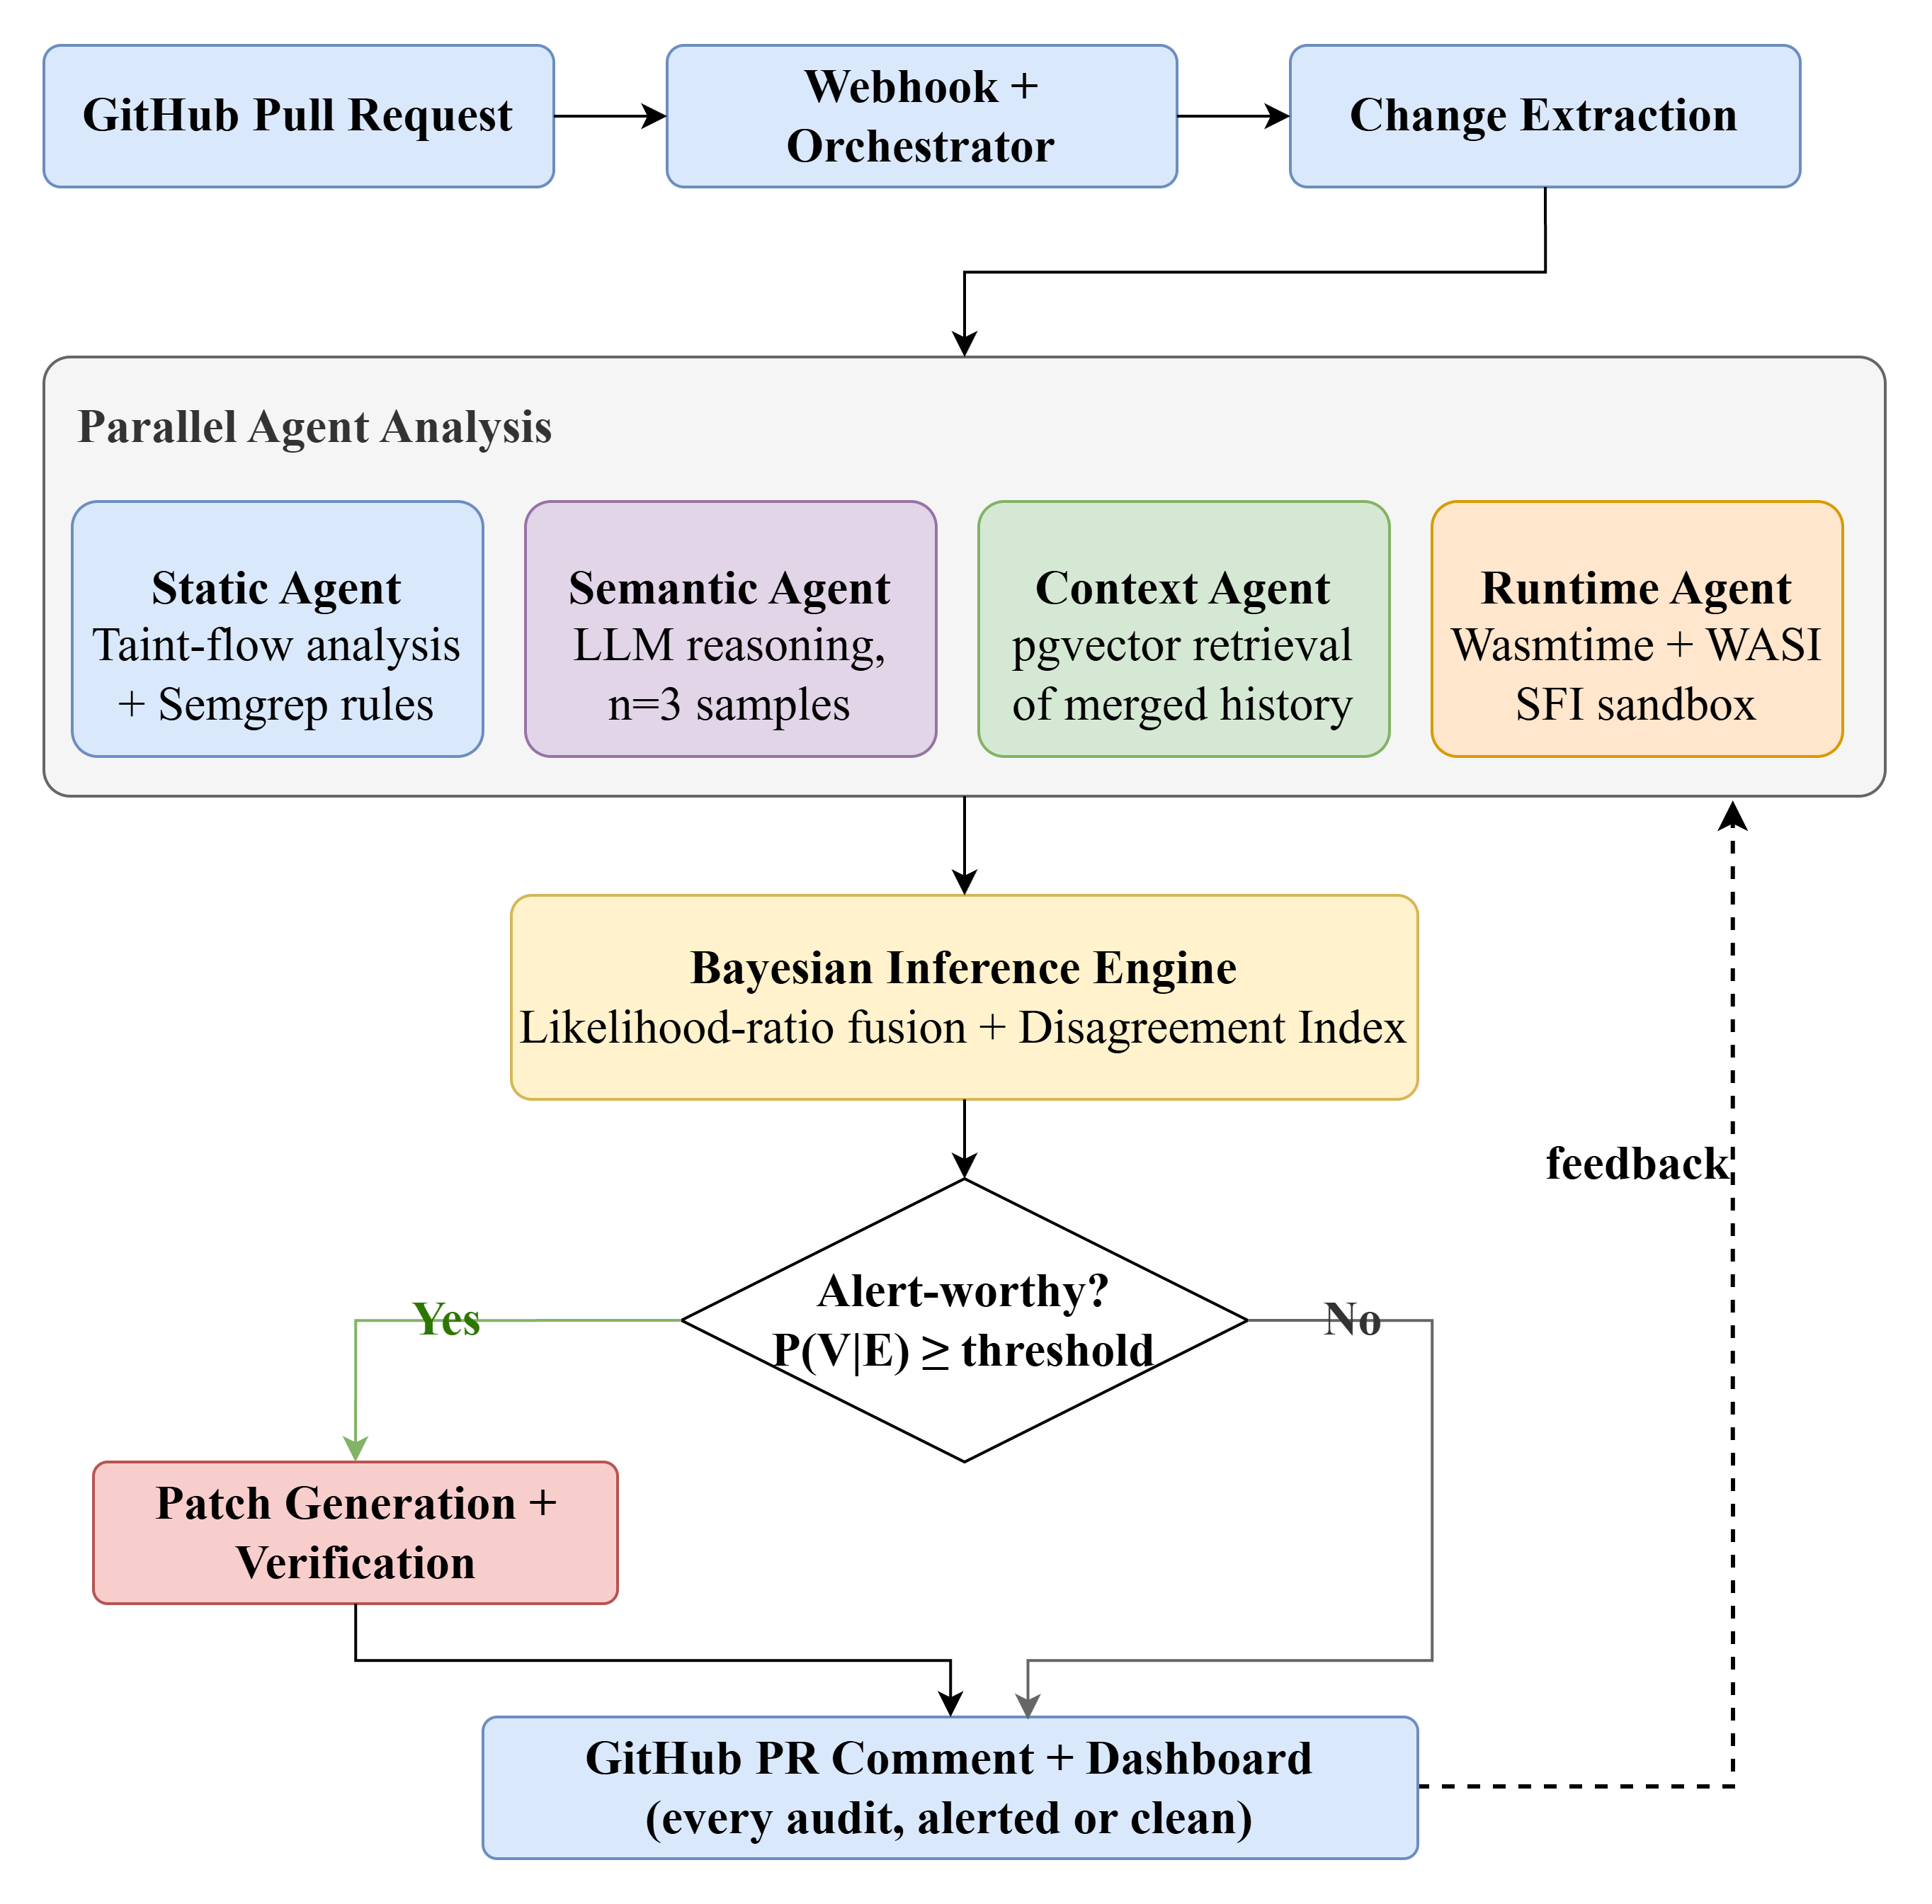
\includegraphics[width=0.78\columnwidth]{codesheriff_workflow.png}
    \caption{Workflow of CodeSheriff.}
    \label{fig:workflow}
\end{figure}

As illustrated in Fig.~\ref{fig:workflow}, the prepared code is analyzed by
four specialized agents: Static, Semantic, Context, and Runtime. Each agent
examines the changes from a different perspective and produces structured
evidence about potential vulnerabilities. The collected evidence is then
passed to a Bayesian Inference Engine, which fuses the agents' likelihood
ratios into a posterior probability and compares it with the fitted alert
threshold to produce the final confidence-aware vulnerability verdict.

When a vulnerability is identified, the patching module generates a
candidate fix, which is re-examined by the deterministic agents before it
is suggested. The audit outcome, comprising the verdict, confidence score,
supporting evidence and, where applicable, patch information, is returned
to both the pull request and the dashboard. As depicted by the feedback
loop in Fig.~\ref{fig:workflow}, merged code is fed back into the agent
analysis stage, so the repository's own history informs the evaluation of
future pull requests.

\section{Implementation Details} \label{IMP}

\subsection{System Architecture}
CodeSheriff is implemented in Python 3.12 as a workspace of nine packages
and three applications, and runs as two processes holding different
credentials. The API process owns the webhook secret and never analyses
code: it verifies the \texttt{X-Hub-Signature-256} header against the raw
request body, writes an audit row, queues the audit identifier and answers
within three seconds, inside GitHub's ten-second limit. The worker process
owns the model key, fetches the changed files, runs the agents and posts
the result. The queued message carries only the identifier, so a
compromised queue discloses no source code. Table~\ref{tab:stack} lists the
technology used at each layer.

\begin{table}[t]
\centering
\caption{Implementation technology stack}
\label{tab:stack}
\footnotesize
\setlength{\tabcolsep}{3pt}
\begin{tabular}{p{1.9cm}p{5.9cm}}
\toprule
Layer & Technology \\
\midrule
API, queue, storage & FastAPI, Celery, Redis, PostgreSQL 16 with pgvector \\
Parsing       & tree-sitter for extraction, \texttt{ast} for patch checks \\
Structural    & Custom taint engine over networkx, Semgrep~\cite{semgrep} \\
Semantic      & Hosted Gemini Flash-Lite model, $n=3$ samples \\
Context       & Sentence-Transformers \texttt{bge-small-en-v1.5}, 384-dim \\
Runtime       & Wasmtime with WASI, CPython 3.12 built to WebAssembly \\
Dashboard     & Next.js, TypeScript, Tailwind, Recharts \\
Quality gates & 1249 tests, \texttt{mypy --strict}, \texttt{ruff}, import-linter \\
\bottomrule
\end{tabular}
\end{table}

\subsection{Agent Interface and Isolation}
Every agent implements exactly one function, shown in
Fig.~\ref{fig:contract}. An agent may import the shared contract package
and nothing else: not a sibling agent, the fusion engine, the database or
the labelled corpus. These boundaries are checked by
\texttt{import-linter} in the build, so the agent independence assumed by
(\ref{eq:post}) is enforced mechanically rather than by convention. An
agent never raises: every failure path returns an abstention with a
distinct reason, and returning an empty list is a defect, because it is
indistinguishable from silence.

\begin{figure}[t]
\centering
\footnotesize
\begin{verbatim}
# the contract every agent implements
def analyze(unit: ChangeUnit) -> list[Evidence]:
    ...
# three statements, never an empty list
Evidence.detection(cwe, raw_score, key)
Evidence.silence(covered_cwes)
Evidence.abstention(reason)
\end{verbatim}
\caption{The agent contract. One function, three kinds of statement.}
\label{fig:contract}
\end{figure}

\subsection{Sandbox Configuration}
The Runtime Agent loads a pinned CPython build compiled to WebAssembly and
verifies its SHA-256 digest before use; a mismatch is fatal. Capabilities
are absent rather than filtered, so \texttt{os.environ} is empty because
nothing was inherited, and WASI preview~1 defines no socket call, so a
module asking to open a network connection fails to instantiate. Each run
is bounded by fuel, wall-clock time and memory, and each unit gets a fresh
store. Without the interpreter the agent abstains per unit at $\Lambda=1$
rather than failing the audit.

\subsection{Ground-Truth Corpus and Protocol}
Calibration can only be measured against ground truth, so the evaluation
uses a hand-written corpus of 76 Python functions arranged as 38
\emph{twin pairs}: the same function once vulnerable and once fixed, which
makes a false positive directly visible as a detection on the safe twin.
The corpus covers ten weakness classes of the Common Weakness Enumeration
(CWE): 22, 78, 79, 89, 94, 502, 639, 798, 862 and 918. Pairs, not
individual cases, are assigned to splits, so twins never straddle one: 46
units for calibration, 14 for validation and 16 held out for test. The
protocol is fixed in advance: ratios are fitted only on calibration, the
threshold is selected only on validation, and the test split is evaluated
exactly once at the end. Because every case has a twin, corpus prevalence
is $0.5$ by construction, which is not a property of real pull requests;
the prior is therefore declared as $\pi=0.03$ and all metrics are weighted
so that vulnerable claims carry $3\%$ of the weight.

\section{Result Analysis and Discussion} \label{RES}

\subsection{Experimental Setup and Metrics}
Experiments were run on a system with 16~GB RAM and an Intel Core i5
processor. Evaluation replays committed model responses, so every number is
reproducible without a network call. A statement about one weakness in one
unit is called a \emph{claim}: the calibration split yields 49 claims and
the validation split 15, of which 7 are vulnerable.

Detection quality is reported as precision (P), recall (R) and $F_1$.
Reliability is reported with the Brier score~\cite{brier1950} and the
expected calibration error (ECE)~\cite{guo2017calibration}:
\begin{equation}
\mathrm{Brier}=\frac{1}{N}\sum_{i=1}^{N}\left(p_i-y_i\right)^2,\quad
\mathrm{ECE}=\sum_{b=1}^{10}\frac{|B_b|}{N}\bigl|\mathrm{freq}_b-\mathrm{conf}_b\bigr|
\label{eq:metrics}
\end{equation}
where $p_i$ is the predicted probability of claim $i$, $y_i\in\{0,1\}$ its
true label, and $B_b$ the set of claims whose probability falls in bin $b$.
Both are zero for a perfect system and both must be read together, as
shown below.

\subsection{Per-Agent Detection Results}
Each agent was first measured alone on the calibration split, over the
cases the corpus predicts it can detect and over all safe twins. The three
deterministic agents reached full recall in their own scope with no false
positive: 13/13 cases for the Structural Agent over 23 safe twins, 5/5 for
the Context Agent over 11 twins, and 9/9 for the Runtime Agent over 23
twins. The Semantic Agent is measured differently, because a language model
fails in ways a rule cannot: none of its accepted findings quoted a sink
absent from the code, no instruction injected into the analysed code
changed its answer, and it correctly reported nothing on $94\%$ of safe
twins.

\subsection{Fitted Likelihood Ratios}
Table~\ref{tab:lr} lists the ratios fitted with (\ref{eq:lr}) on the
calibration split. A medium structural detection multiplies the odds of a
vulnerability by $15.56$, while structural silence divides them by about
$15$. Two cells are worth noting: a low or medium semantic detection, that
is a weakness reported by only one or two of the three samples, has a ratio
below $1$ and is therefore evidence of \emph{safety}. A voting scheme would
count such a report as a ``yes'' vote; the fitted ratio records what the
data shows instead.

\begin{table}[t]
\centering
\caption{Fitted likelihood ratios per agent and evidence cell
(--: cell never observed, contributes exactly $1.0$)}
\label{tab:lr}
\small
\setlength{\tabcolsep}{5pt}
\begin{tabular}{lcccc}
\toprule
Agent & \textsc{high} & \textsc{medium} & \textsc{low} & \textsc{silence} \\
\midrule
Structural & 2.22 & 15.56 & --   & 0.065 \\
Semantic   & 9.48 & 0.56  & 0.74 & 0.304 \\
Context    & 2.00 & 4.00  & 2.00 & 0.167 \\
Runtime    & 6.92 & --    & --   & 0.115 \\
\bottomrule
\end{tabular}
\end{table}

\subsection{Comparative Analysis}
CodeSheriff is compared with two inference baselines that consume the
\emph{same} agent evidence, so the only difference is how it is combined.
\emph{Majority vote} scores a claim by the share of agents that detected,
ignoring abstentions, which is what voting offers in place of a
probability; \emph{prior only} ignores the agents and always predicts the
$3\%$ base rate. All three use $\tau=0.227$.
Table~\ref{tab:comparison} reports both splits and
Fig.~\ref{fig:compare}(a) plots the validation split.

\begin{table}[t]
\centering
\caption{Detection and calibration using identical agent evidence.
Best per column in bold.}
\label{tab:comparison}
\small
\setlength{\tabcolsep}{3.2pt}
\begin{tabular}{llccccc}
\toprule
Split & System & ECE $\downarrow$ & Brier $\downarrow$ & P $\uparrow$ & R $\uparrow$ & $F_1$ $\uparrow$ \\
\midrule
Valid.
 & Prior only        & \textbf{0.000} & 0.029 & 0.000 & 0.000 & 0.000 \\
 & Majority vote     & 0.141 & 0.059 & 0.076 & \textbf{1.000} & 0.142 \\
 & CodeSheriff       & 0.027 & \textbf{0.013} & \textbf{1.000} & 0.857 & \textbf{0.923} \\
\midrule
Calib.
 & Prior only        & \textbf{0.000} & 0.029 & 0.000 & 0.000 & 0.000 \\
 & Majority vote     & 0.092 & 0.068 & 0.161 & \textbf{0.957} & 0.276 \\
 & CodeSheriff       & 0.009 & \textbf{0.010} & \textbf{1.000} & 0.696 & \textbf{0.821} \\
\bottomrule
\end{tabular}
\end{table}

\begin{figure}[t]
\centering
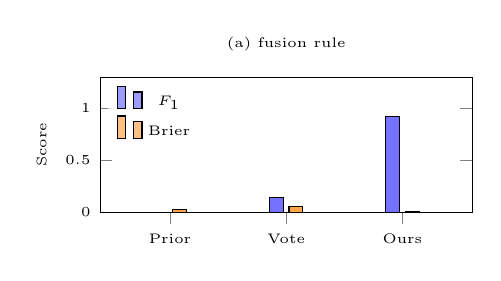
\begin{tikzpicture}
\begin{axis}[
  ybar, width=0.52\columnwidth, height=3.3cm,
  bar width=5pt, enlarge x limits=0.3,
  ymin=0, ymax=1.3, ytick={0,0.5,1},
  symbolic x coords={Prior,Vote,Ours},
  xtick=data, xtick pos=left, tick label style={font=\tiny},
  ylabel={Score}, ylabel style={font=\tiny},
  title={(a) fusion rule}, title style={font=\tiny},
  legend columns=1,
  legend style={font=\tiny, at={(0.02,0.98)}, anchor=north west, draw=none,
                fill opacity=0.7, text opacity=1}]
\addplot[fill=blue!55]   coordinates {(Prior,0) (Vote,0.142) (Ours,0.923)};
\addplot[fill=orange!70] coordinates {(Prior,0.029) (Vote,0.059) (Ours,0.013)};
\legend{$F_1$, Brier}
\end{axis}
\end{tikzpicture}\hfill
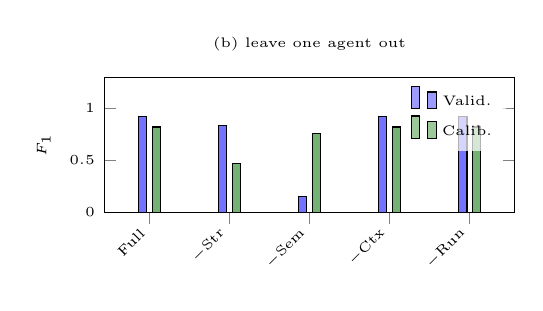
\begin{tikzpicture}
\begin{axis}[
  ybar, width=0.56\columnwidth, height=3.3cm,
  bar width=3pt, enlarge x limits=0.14,
  ymin=0, ymax=1.3, ytick={0,0.5,1},
  symbolic x coords={Full,$-$Str,$-$Sem,$-$Ctx,$-$Run},
  xtick=data, xtick pos=left,
  tick label style={font=\tiny}, x tick label style={rotate=45, anchor=east},
  ylabel={$F_1$}, ylabel style={font=\tiny},
  title={(b) leave one agent out}, title style={font=\tiny},
  legend columns=1,
  legend style={font=\tiny, at={(0.98,0.98)}, anchor=north east, draw=none,
                fill opacity=0.7, text opacity=1}]
\addplot[fill=blue!55] coordinates {(Full,0.923) ($-$Str,0.833) ($-$Sem,0.157) ($-$Ctx,0.923) ($-$Run,0.923)};
\addplot[fill=green!45!black!55] coordinates {(Full,0.821) ($-$Str,0.473) ($-$Sem,0.757) ($-$Ctx,0.821) ($-$Run,0.821)};
\legend{Valid., Calib.}
\end{axis}
\end{tikzpicture}
\caption{(a) Detection quality and calibration error for the three fusion
rules on the validation split. (b) $F_1$ after removing one agent at a
time, on both splits.}
\label{fig:compare}
\end{figure}

CodeSheriff attains an $F_1$ of $0.923$ at a precision of $1.000$, alerting
on 6 of 15 claims. Majority voting over identical evidence reduces $F_1$ to
$0.142$ and raises ECE from $0.027$ to $0.141$: with no prior to moderate a
single agent's alert, it finds every vulnerability but most of its ten
alerts are false. The prior-only baseline reaches ECE $=0.000$ by detecting
nothing, which shows ECE alone is insufficient; its Brier score of $0.029$,
more than twice CodeSheriff's $0.013$, exposes the difference. The same
ordering holds on the larger calibration split.

\subsection{Calibration Quality}
Fig.~\ref{fig:reliability} plots, for each probability bin on the
validation split, the mean predicted probability against the observed share
of vulnerable claims; a perfectly calibrated system lies on the diagonal.
Most claims receive a very low probability and are indeed safe, and every
high-probability claim is vulnerable. Two middle bins lie above the
diagonal, so the system was slightly \emph{under}-confident there: claims
reported at $0.23$ and $0.34$ were vulnerable. Those bins hold one or two
claims each and contribute little to the ECE; judging that region reliably
requires a larger corpus.

\begin{figure}[t]
\centering
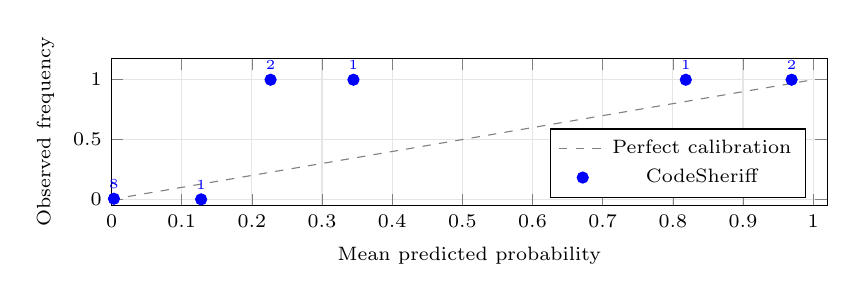
\begin{tikzpicture}
\begin{axis}[
  width=0.88\columnwidth, height=3.45cm,
  xmin=0, xmax=1.02, ymin=-0.05, ymax=1.18,
  xlabel={Mean predicted probability}, ylabel={Observed frequency},
  label style={font=\scriptsize}, tick label style={font=\scriptsize},
  legend style={font=\scriptsize, at={(0.97,0.05)}, anchor=south east},
  grid=major, grid style={gray!20}]
\addplot[dashed, gray, domain=0:1] {x};
\addplot[only marks, mark=*, blue, mark size=2pt,
  nodes near coords, point meta=explicit symbolic,
  every node near coord/.append style={font=\tiny, anchor=south}]
  coordinates {
  (0.0034,0.0050) [8]
  (0.1277,0.0)    [1]
  (0.2267,1.0)    [2]
  (0.3448,1.0)    [1]
  (0.8185,1.0)    [1]
  (0.9693,1.0)    [2]};
\legend{Perfect calibration, CodeSheriff}
\end{axis}
\end{tikzpicture}
\caption{Reliability diagram on the validation split. Labels give the
number of claims in each bin.}
\label{fig:reliability}
\end{figure}

\subsection{Threshold Selection}
The threshold was selected on the validation split by sweeping every
distinct posterior value and keeping the best weighted $F_1$. Below
$0.227$ recall is complete, but one safe claim at $0.13$ is alerted, and
because safe code dominates in production that single false alarm drives
weighted precision to $0.175$ and $F_1$ to $0.291$. Above $0.227$ precision
stays at $1.000$ while recall falls to $0.571$ at $\tau=0.345$ and $0.286$
at $\tau=0.969$, so $\tau=0.227$ is the balance point. These figures are
selection-time estimates, not held-out measurements.

\subsection{Ablation Study}
Each agent was removed in turn to isolate its contribution. A removed agent
contributes an abstention at likelihood ratio $1.0$, so the posterior
changes only through the evidence it no longer supplies.
Table~\ref{tab:ablation} reports both splits, and Fig.~\ref{fig:compare}(b)
plots the resulting $F_1$.

\begin{table}[t]
\centering
\caption{Leave-one-agent-out ablation at $\tau=0.227$}
\label{tab:ablation}
\small
\setlength{\tabcolsep}{3pt}
\begin{tabular}{lcccccc}
\toprule
 & \multicolumn{3}{c}{Validation split} & \multicolumn{3}{c}{Calibration split} \\
\cmidrule(lr){2-4}\cmidrule(lr){5-7}
Configuration & ECE & Brier & $F_1$ & ECE & Brier & $F_1$ \\
\midrule
Full model     & 0.027 & 0.013 & \textbf{0.923} & 0.009 & 0.010 & \textbf{0.821} \\
$-$ Structural & 0.012 & 0.015 & 0.833 & 0.007 & 0.017 & 0.473 \\
$-$ Semantic   & 0.047 & 0.031 & 0.157 & 0.011 & 0.015 & 0.757 \\
$-$ Context    & 0.026 & 0.013 & 0.923 & 0.007 & 0.011 & 0.821 \\
$-$ Runtime    & 0.028 & 0.013 & 0.923 & 0.011 & 0.011 & 0.821 \\
\bottomrule
\end{tabular}
\end{table}

The two splits disagree about which agent matters most, and that
disagreement is itself the main finding. On validation, removing the
Semantic Agent costs $0.766$ in $F_1$ and collapses precision to $0.096$;
on calibration, removing the Structural Agent is the most damaging, costing
$0.348$ in $F_1$ as precision falls to $0.359$, while the Semantic Agent
costs only $0.064$ there. No single agent is sufficient on both splits,
which is the empirical case for heterogeneous agents. Removing the Context
or Runtime Agent leaves every decision unchanged; this is a null result
rather than redundancy, since both have deliberately narrow scopes and
usually confirm a decision another agent has already reached, while still
moving the posterior: calibration ECE rises from $0.009$ to $0.011$ without
the Runtime Agent.

\subsection{Comparison with Related Systems}
A direct numerical comparison with published systems is not meaningful,
because they are evaluated on different languages, weakness sets and metric
protocols. MAVUL~\cite{ref16}, the closest multi-agent precedent, targets
C/C++ memory-safety CWEs under its own P-C/P-V/P-B/P-R protocol and reports
no reliability measure; DeepSecure~\cite{ref2} is a Python-specific hybrid
deep-learning detector with a confidence component but no repository
context or execution evidence; AegisGuard~\cite{ref1} adds context and risk
stratification; and Reddy \textit{et al.}~\cite{ref6} triage with
knowledge-based agents. Table~\ref{tab:related} therefore compares
capabilities rather than scores. To our knowledge, CodeSheriff is the first
of these to combine four different techniques with a calibrated
probability, sandboxed execution and verified patch suggestions inside the
pull-request workflow.

\begin{table}[t]
\centering
\caption{Capability comparison with related systems
($\checkmark$: reported; --: not reported in the cited work)}
\label{tab:related}
\small
\setlength{\tabcolsep}{3pt}
\begin{tabular}{lccccc}
\toprule
Capability & \cite{ref2} & \cite{ref1} & \cite{ref16} & \cite{ref6} & Ours \\
\midrule
Multiple agents              & --  & --  & $\checkmark$ & $\checkmark$ & $\checkmark$ \\
Distinct technique per agent & --  & --  & --  & --  & $\checkmark$ \\
Calibrated confidence        & $\checkmark$ & --  & --  & --  & $\checkmark$ \\
Repository context           & --  & $\checkmark$ & $\checkmark$ & --  & $\checkmark$ \\
Sandboxed execution          & --  & --  & --  & --  & $\checkmark$ \\
Verified patch in the PR     & --  & --  & --  & --  & $\checkmark$ \\
\bottomrule
\end{tabular}
\end{table}

\subsection{Assumptions and Limitations}
\label{subsec:limitations}
The corpus is Python-only, self-authored and covers a closed set of ten
CWEs, so the reported rates describe this corpus and not arbitrary pull
requests. The validation split, at 15 claims, is too small for a meaningful
confidence interval, and the threshold was selected on it; the held-out
test split remains unevaluated. Evaluation is a single deterministic run
against committed model recordings, so no sampling variance is reported.
Semgrep has no build for the fitting platform, so the structural ratios in
Table~\ref{tab:lr} describe a one-backend agent. Finally, the $3\%$ base
rate is declared rather than measured.

\section{Conclusion and Future Scope} \label{CON}

\subsection{Conclusion}
This paper presented CodeSheriff, a heterogeneous multi-agent security
auditor for GitHub pull requests that fuses structural, semantic,
contextual and runtime evidence through Bayesian inference rather than
majority voting. The design keeps the four agents independent, separates an
agent that found nothing from one that could not run, and fits every
likelihood ratio and the alert threshold on labelled data. On the
validation split it attained an $F_1$ of $0.923$ at a precision of $1.000$
with an expected calibration error of $0.027$, outperforming a
majority-vote combiner over identical evidence by a factor of $6.5$ in
$F_1$ while reducing calibration error five-fold, and the ablation showed
that no single agent accounts for this. Unlike existing detectors, which
report a verdict with no reliability measure, its central contribution is a
posterior probability that is simultaneously discriminative and calibrated,
verified jointly through $F_1$ and the Brier score, and accompanied by
patch suggestions that pass a fixed verification ladder.

\subsection{Future Scope}
Several directions follow from Section~\ref{subsec:limitations}. The
structural agent must be re-observed on a Linux or CI environment where
both of its backends are available, since the current fit describes a
one-backend agent, and the held-out test split should then be scored
exactly once under the protocol of Section~\ref{IMP}. Scoring Semgrep,
Bandit and a single-pass LLM under the same weighted protocol would
complete the external comparison, and enlarging the corpus with real
vulnerability-fixing commits would allow interval estimation and a
sensitivity analysis over the threshold and the declared base rate.
Finally, extending language coverage to JavaScript and TypeScript, which
the tree-sitter based extraction already permits, evaluating a fine-tuned
semantic model against the hosted one, and using the same sandbox to
release CI/CD secrets only to verified code are identified as future work.

% \nocite{*}
\balance
\addcontentsline{toc}{section}{References}
\bibliographystyle{IEEEtran}
\bibliography{references}

\end{document}
